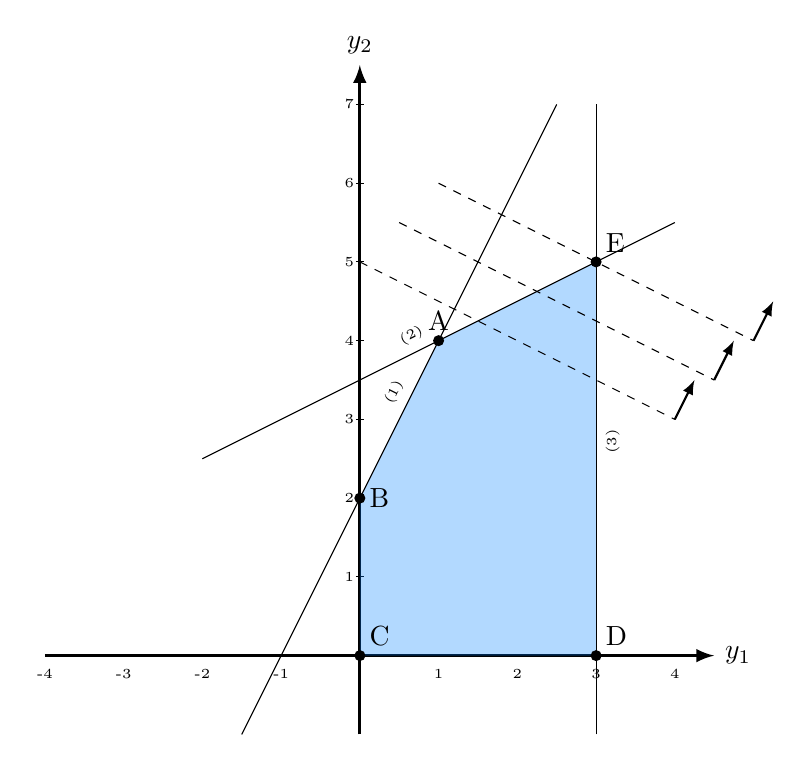
\begin{tikzpicture}
  \draw[very thick, -latex] (0, 1) coordinate(x1) -- (8.5, 1) coordinate(x2) node[right] {$y_1$};
  \draw[very thick, -latex] (4, 0) coordinate(y1) -- (4, 8.5) coordinate(y2) node[above] {$y_2$};
  \foreach \x in {-4, ..., -1} {
    \draw (\x+4, 0.95) -- (\x+4, 0.95) node[below] {\tiny\x};
  }
  \foreach \x in {1, ..., 4} {
    \draw (\x+4, 0.95) -- (\x+4, 0.95) node[below] {\tiny\x};
  }
  \foreach \y in {1, ..., 7} {
    \draw (3.95, \y+1) -- (4.05, \y+1) node[left] {\tiny\y};
  }
  \fill[blue!50!cyan, opacity=0.3] (4, 1) -- (4, 3) -- (5, 5) -- (7, 6) -- (7, 1) -- cycle;    
  \draw (2.5, 0) coordinate (a1) --
    node[above right, sloped] {\tiny $(1)$} (6.5, 8) coordinate (a2);
  
  \draw (2, 3.5) coordinate (b1) --
    node[above left, sloped] {\tiny $(2)$} (8, 6.5) coordinate (b2);
  
  \draw (7, 0) coordinate (c1) --
    node[below left, sloped] {\tiny $(3)$} (7, 8) coordinate (c2);
  
  \coordinate (v1) at (intersection of a1--a2 and b1--b2);
  \coordinate (v2) at (intersection of a1--a2 and y1--y2);
  \coordinate (v3) at (intersection of x1--x2 and y1--y2);
  \coordinate (v4) at (intersection of x1--x2 and c1--c2);
  \coordinate (v5) at (intersection of b1--b2 and c1--c2);
  \fill[black] (v1) node[above] {A} circle (2pt);
  \fill[black] (v2) node[right] {B} circle (2pt);
  \fill[black] (v3) node[above right] {C} circle (2pt);
  \fill[black] (v4) node[above right] {D} circle (2pt);
  \fill[black] (v5) node[above right] {E} circle (2pt);
  
  \draw[dashed] (4, 6) coordinate (b1) -- (8, 4) coordinate (b2);
  \draw[dashed] (4.5, 6.5) coordinate (b1) -- (8.5, 4.5) coordinate (b2);
  \draw[dashed] (5, 7) coordinate (b1) -- (9, 5) coordinate (b2);
		
  \draw[-latex, thick] (8, 4)--(8.25, 4.5);
  \draw[-latex, thick] (8.5, 4.5)--(8.75, 5);
  \draw[-latex, thick] (9, 5)--(9.25, 5.5);
\end{tikzpicture}


